%!TEX root = pset2.tex

\section{Support Vector Machine}\label{sec:svm}

Support Vector Machines are a popular classification method to construct linear or nonlinear decision boundaries
by solving a convex optimization problem.  There are two common forms of the optimization problem considered for SVM,
which we refer to as the primal and dual.  In this paper, we only consider the dual form, because it is computationally more tractable
for many problems, and this method has the ability to generalize to different choices of kernel.  The dual form of SVM for a general
kernel function $k: \mathcal{X} \times \mathcal{X} \rightarrow \mathbb{R}$ is as follows:

\begin{equation}
\label{eq:svm_dual}
\begin{array}{rll}
\underset{\alpha \in \mathbb{R}^n}{\max}~ & \sum\limits_{i = 1}^n \alpha_i 
- \frac{1}{2} \sum\limits_{i = 1}^n\sum\limits_{j = 1}^n \alpha_i \alpha_j y^{(i)} y^{(j)} k(x^{(i)}, x^{(j)}) \vspace{3pt}\\
\textup{s.t.}~ & 0 \leq \alpha_i \leq C,&~~~i=1,\ldots ,n, \vspace{3pt}\\
& \sum\limits_{i = 1}^n \alpha_i y^{(i)} = 0. & \\
\end{array}
\end{equation}

\subsection{Implementation}

First, we implemented the dual form of the SVM with a linear kernel, where $k$ is the usual dot product $k(x, z) = \langle x,z \rangle$ for all $x, z \in \mathcal{X}$. 
In MATLAB, we created a function with inputs: data $X \in \mathbb{R}^{n \times p}$, labels $Y \in \{-1,1\}$, and cost parameter $C \in \mathbb{R}^{+}$. 
Within the function, we use the quadratic solver \texttt{quadprog} to solve the SVM dual problem (\ref{eq:svm_dual}) with these parameters to find the optimal $\alpha$'s.
Since \texttt{quadprog} requires that the problem fit into a certain functional form, we reformulate the problem (\ref{eq:svm_dual}) as follows:

\begin{equation}
\label{eq:svm_dual2}
\begin{array}{rll}
-\underset{\alpha \in \mathbb{R}^n}{\min}~ & \frac{1}{2} \alpha^T H \alpha - \sum\limits_{i = 1}^n \alpha_i \vspace{3pt}\\
\textup{s.t.}~ & 0 \leq \alpha_i \leq C,&~~~i=1,\ldots ,n, \vspace{3pt}\\
& \sum\limits_{i = 1}^n \alpha_i y^{(i)} = 0, & \vspace{5pt}\\
\end{array}
\end{equation}
where:  $H \in \mathbb{R}^{n \times n}$ is a matrix with $(i,j)^{th}$ entry $H_{ij} = y^{(i)} y^{(j)} k(x^{(i)}, x^{(j)})$.  Given the optimal solution $\alpha \in \mathbb{R}^n$ for the SVM problem with a linear kernel, the chosen linear decision boundary $\theta^T x + \theta_0 = 0$ is given by:

\begin{equation}
\label{eq:svm_theta}
\theta = \sum\limits_{i = 1}^n \alpha_i y^{(i)} x^{(i)}
\end{equation}
\begin{equation}
\label{eq:svm_theta_0}
\theta_0 = \frac{1}{\mathcal{M}} \Big(\sum\limits_{j \in \mathcal{M}} \Big(y^{(j)} - \sum\limits_{i \in \mathcal{S}}\alpha_i y^{(i)} (x^{(j)})^T x^{(i)} \Big)\Big)
\end{equation}
where ${\Cal M} = \{i : 0 < \alpha_i < C\}$ and ${\Cal S} = \{i : \alpha_i > 0\}$.
The output of our linear SVM function is $[\theta, \theta_0]$.  We tested our function on the 2D example $X = \{(1,2),(2,2),(0,0),(-2,3)\}$, $Y = \{1,1,-1,-1\}$.  
For this problem, the objective function generated for minimization problem (\ref{eq:svm_dual2}) is:

\begin{equation}
\label{eq:svm_objective1}
\frac{1}{2} \alpha^T H \alpha - \sum\limits_{i = 1}^4 \alpha_i,
\end{equation}
where:
\[
H = \begin{bmatrix}
     5   &  6  &   0  &  -4 \\
     6   &  8  &   0  &  -2 \\
     0   &  0  &   0  &   0 \\
    -4   & -2  &  0  &   13 \\
\end{bmatrix}
\]

The constraints are:
%
\begin{equation}
0 \leq \alpha_i \leq C,~~~i=1,\ldots ,4,
\end{equation}
\begin{equation}
\alpha_1 + \alpha_2 - \alpha_3 - \alpha_4 = 0.
\end{equation}

\subsection{Performance on datasets}

We tested our linear SVM function on the same 2D datasets from the previous section, with parameter $C = 1$.  The estimated coefficients are listed in Table \ref{tab:SVM_reg_coeff}.

\begin{table}[h!]
\centering
\caption{Estimated SVM coefficients and accuracy, $C = 1$ }
\begin{tabular}{lrrrrrr}
  \hline\hline
  Data   & $w_0$ 	& $w_1$ 	  & $w_2$ 	& Train accuracy & Valid accuracy & Test accuracy\\
  \hline
  stdev1 & 1.2333    &1.2409   & -0.4204         & 1.0000    &1.0000     & 0.9975\\
  stdev2 & 0.4573    & 0.7552   & -0.1410        & 0.9050    & 0.9200    & 0.9175\\
  stdev4 & 0.1998    & 0.1820   & -0.0470        & 0.7450    & 0.7650    & 0.7800\\
  nonsep &-0.2194   & -0.2118  & -0.4280        & 0.6975    & 0.6950    & 0.7000\\
  \hline\hline
\end{tabular}\label{tab:SVM_reg_coeff}
\end{table}

The decision boundaries at various thresholds are plotted in Figure \ref{fig:SVM_plots}. We observe the following phenomenon:
\begin{enumerate}
\item As data become more linearly non-separable, the accuracy is lower, and the width of the margin increases for the same value of $C$.  
\item In the totally non-separable case, SVM achieves close to 70\% accuracy, which is higher than logistic regression.  These two methods yield different results because they use different loss functions.  SVM uses a hinge loss function which is piecewise linear, while logistic regression uses a logistic loss function which is nonlinear convex.  
\end{enumerate}

\begin{figure}[h!]
\centering
    \begin{subfigure}[b]{0.22\textwidth}
	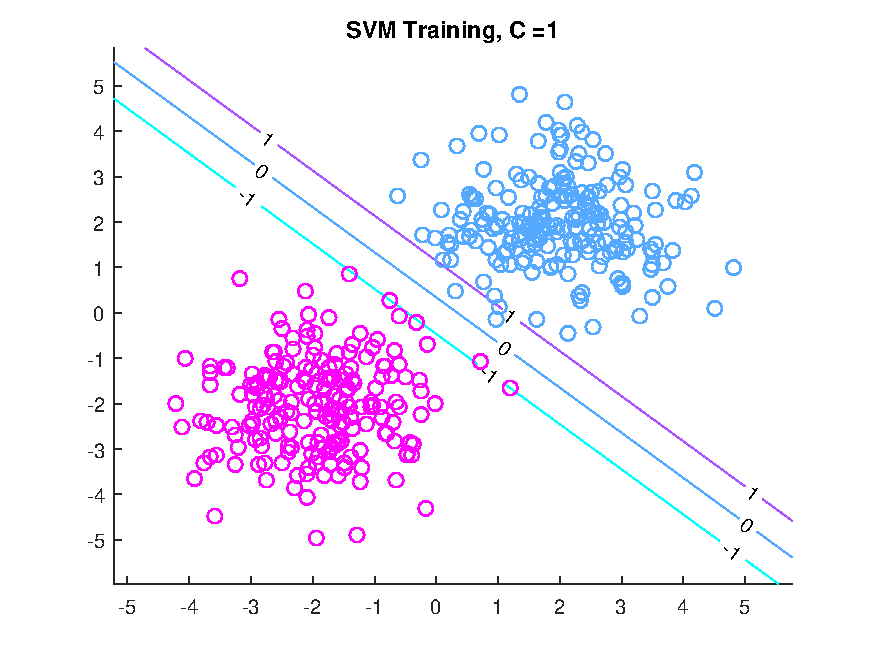
\includegraphics[scale=0.4]{figures/hw2_2_stdev1_a_1.pdf}
	\caption{``stdev1"}\label{fig:svm_data_stdev1a}
    \end{subfigure}
    \quad
    \begin{subfigure}[b]{0.22\textwidth}
	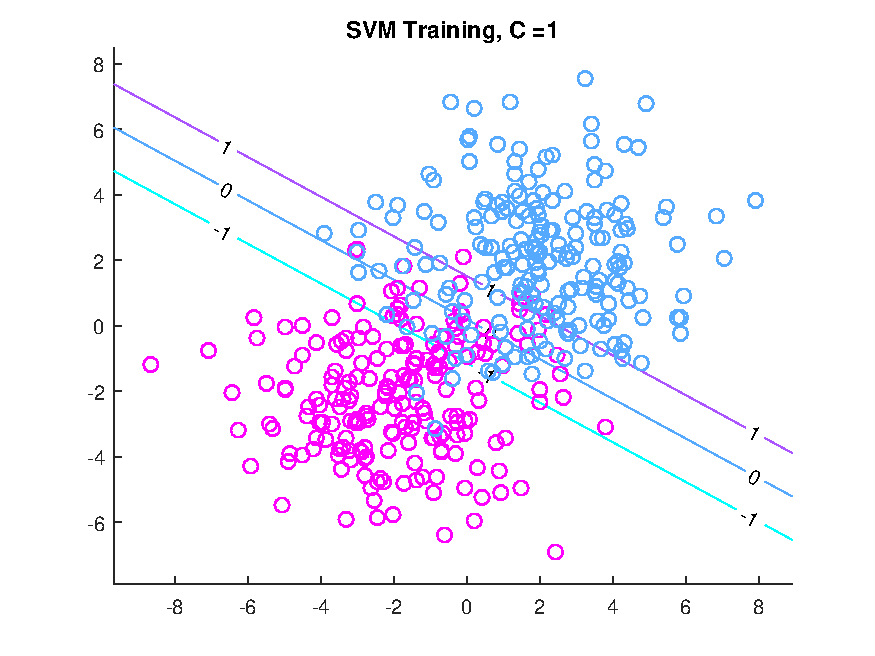
\includegraphics[scale=0.4]{figures/hw2_2_stdev2_a_1.pdf}
	\caption{``stdev2"}\label{fig:svm_data_stdev2a}
    \end{subfigure}
    \quad
    \begin{subfigure}[b]{0.22\textwidth}
	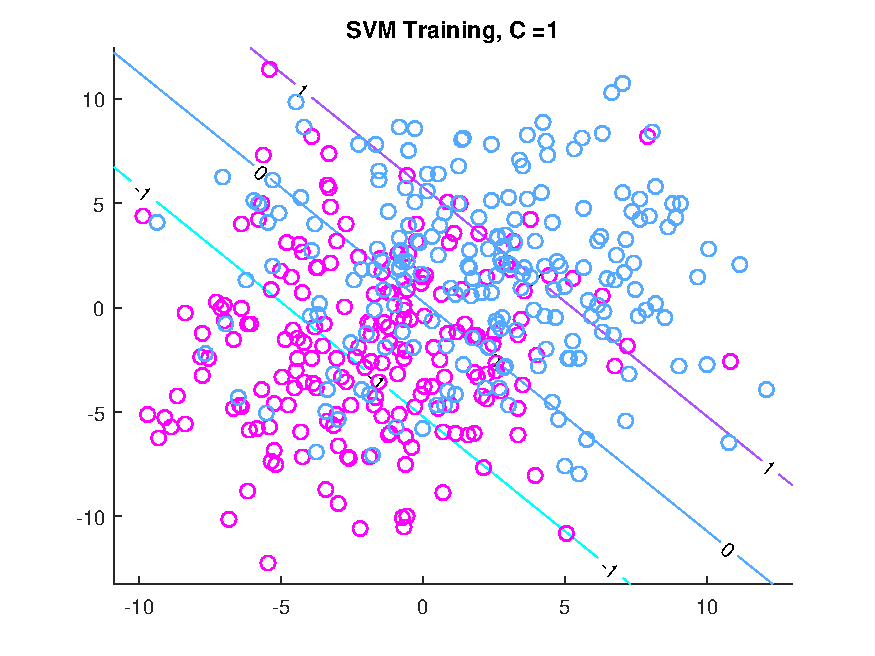
\includegraphics[scale=0.4]{figures/hw2_2_stdev4_a_1.pdf}
	\caption{``stdev4"}\label{fig:svm_data_stdev4a}
    \end{subfigure} 
    \quad
    \begin{subfigure}[b]{0.22\textwidth}
	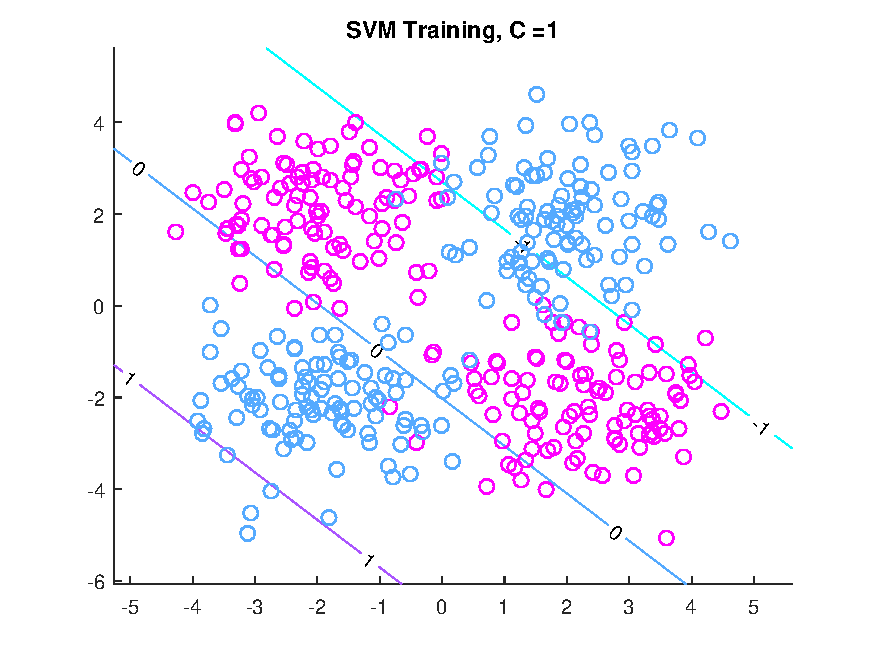
\includegraphics[scale=0.4]{figures/hw2_2_nonsep_a_1.pdf}
	\caption{``nonsep"}\label{fig:svm_data_nonsep_a}
    \end{subfigure}  
    \caption{Plots of decision boundaries from SVM with $C=1$ from training sets.}  \label{fig:SVM_plots}  
\end{figure}

\subsection{Kernel SVM}

We extended our SVM implementation in MATLAB to operate with more general kernels, taking the kernel function or kernel matrix as input.  We tested our SVM method for linear kernel varying $C = \{0.01,0.1,1,10,100\}$, and for gaussian kernel varying $C = \{0.01,0.1,1,10,100\}$ and the squared bandwidth $\sigma^2 = \{0.1,1,10,100\}$.  Plots illustrating the resulting decision boundaries on the 2D datasets for different parameters are shown in Figure \ref{fig:SVM_kernel_plots}.  As $\sigma^2$ decreases, the decision boundary becomes more jagged to fit the training data more exactly.  

%\begin{figure}[h!]
%\centering
%    \begin{subfigure}[b]{0.22\textwidth}
%	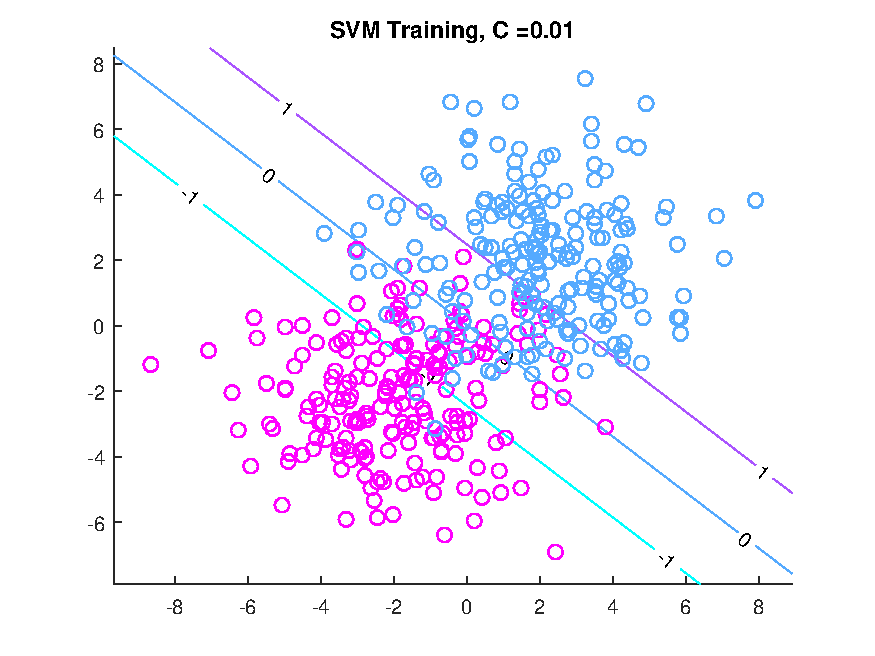
\includegraphics[scale=0.4]{figures/hw2_2_stdev2_a_0_01.pdf}
%	\caption{``stdev1"}\label{fig:svm_data_stdev1a}
%    \end{subfigure}
%    \quad
%    \begin{subfigure}[b]{0.22\textwidth}
%	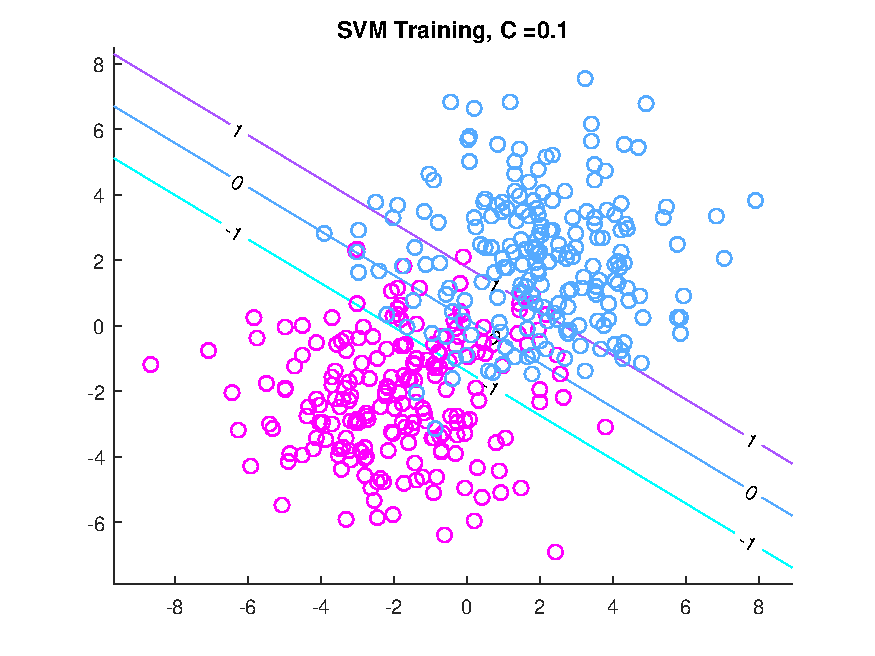
\includegraphics[scale=0.4]{figures/hw2_2_stdev2_a_0_1.pdf}
%	\caption{``stdev2"}\label{fig:svm_data_stdev2a}
%    \end{subfigure}
%    \quad
%    \begin{subfigure}[b]{0.22\textwidth}
%	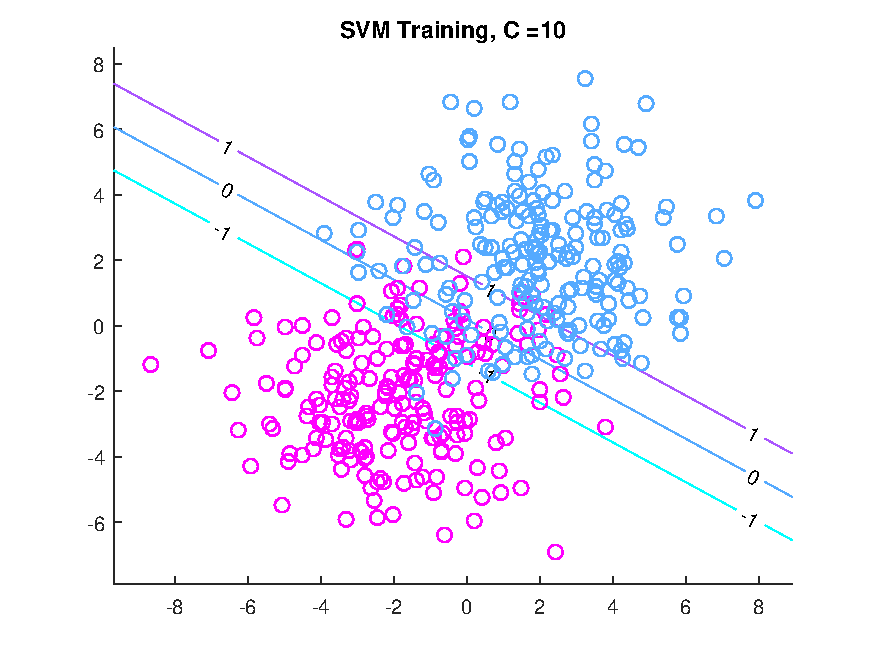
\includegraphics[scale=0.4]{figures/hw2_2_stdev2_a_10.pdf}
%	\caption{``stdev4"}\label{fig:svm_data_stdev4a}
%    \end{subfigure} 
%    \quad
%    \begin{subfigure}[b]{0.22\textwidth}
%	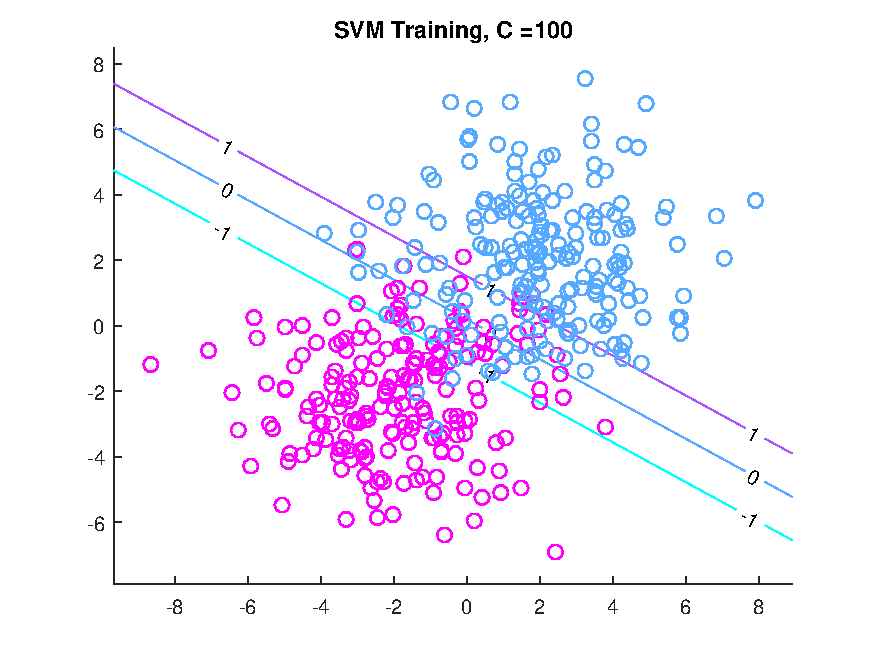
\includegraphics[scale=0.4]{figures/hw2_2_stdev2_a_100.pdf}
%	\caption{``nonsep"}\label{fig:svm_data_nonsep_a}
%    \end{subfigure}  
%    \caption{Plots of decision boundaries from SVM with $C=1$ from training sets.}  \label{fig:SVM_varyC_plots}  
%\end{figure}

\begin{figure}[h!]
\centering
    \begin{subfigure}[b]{0.22\textwidth}
	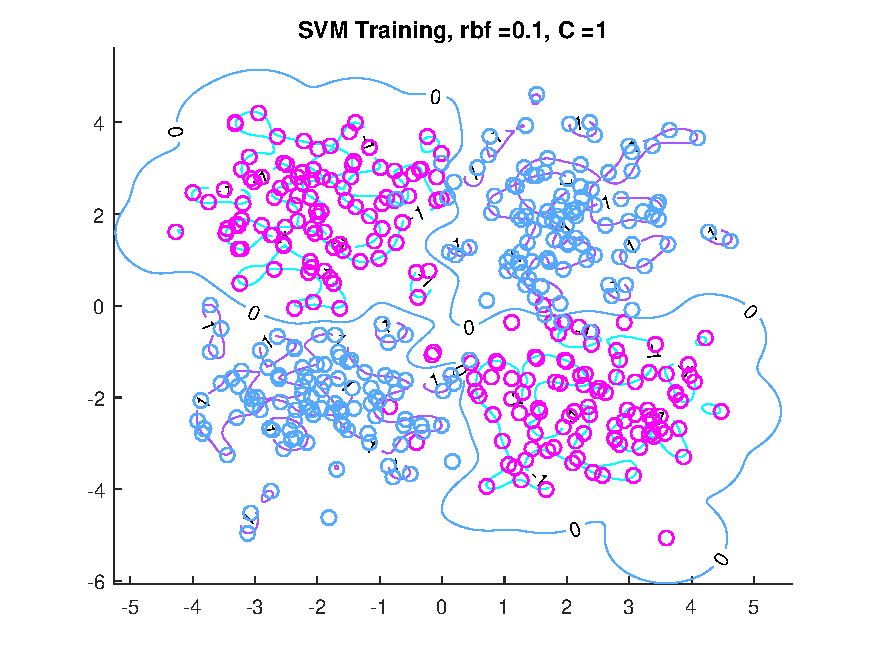
\includegraphics[scale=0.4]{figures/hw2_2_nonsep_rbf_0_1_a_1.pdf}
	\caption{$\sigma^2$ = 0.1}\label{fig:svm_data_stdev1a}
    \end{subfigure}
    \quad
    \begin{subfigure}[b]{0.22\textwidth}
	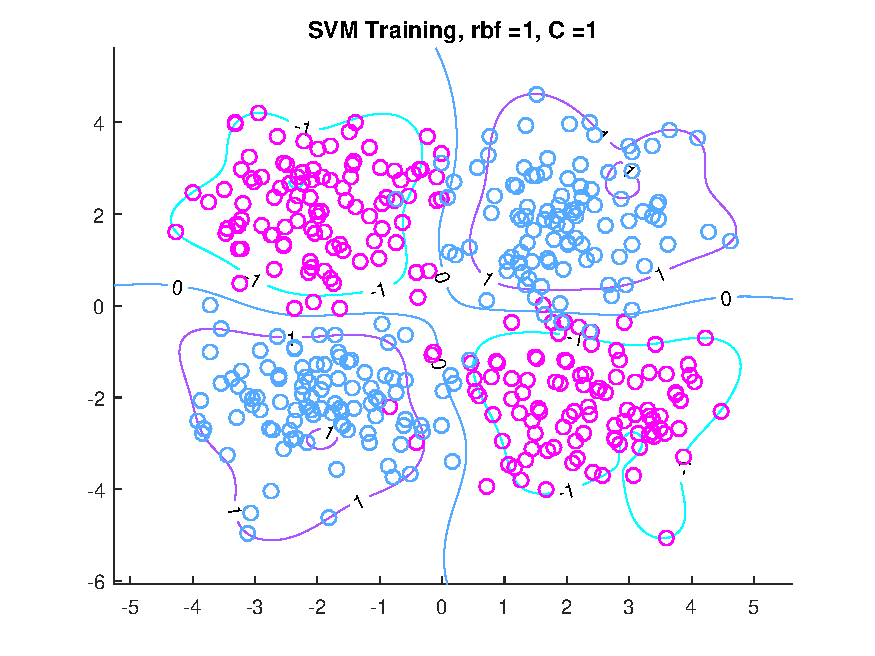
\includegraphics[scale=0.4]{figures/hw2_2_nonsep_rbf_1_a_1.pdf}
	\caption{$\sigma^2$ = 1}\label{fig:svm_data_stdev2a}
    \end{subfigure}
    \quad
    \begin{subfigure}[b]{0.22\textwidth}
	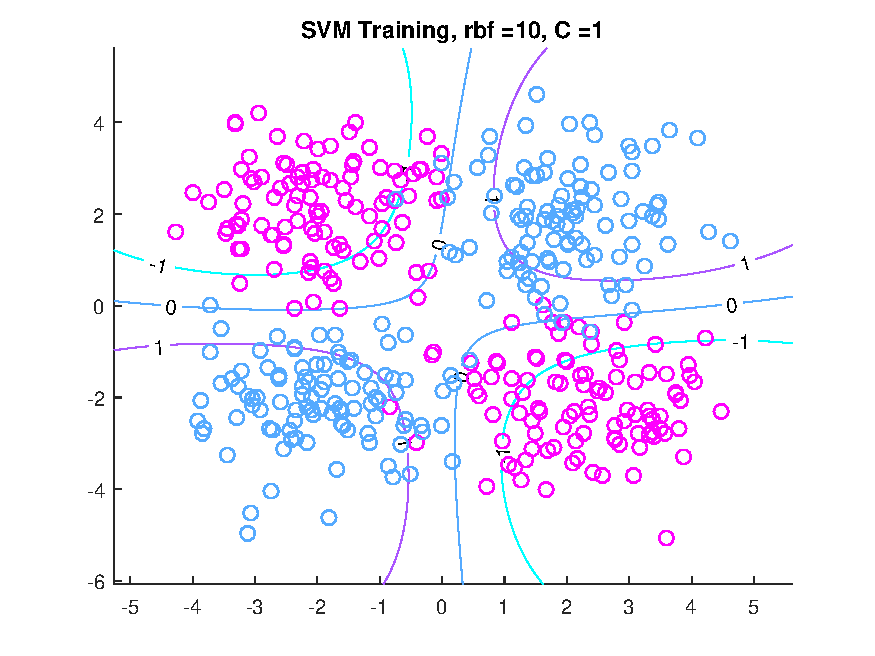
\includegraphics[scale=0.4]{figures/hw2_2_nonsep_rbf_10_a_1.pdf}
	\caption{$\sigma^2$ = 10}\label{fig:svm_data_stdev4a}
    \end{subfigure} 
    \quad
    \begin{subfigure}[b]{0.22\textwidth}
	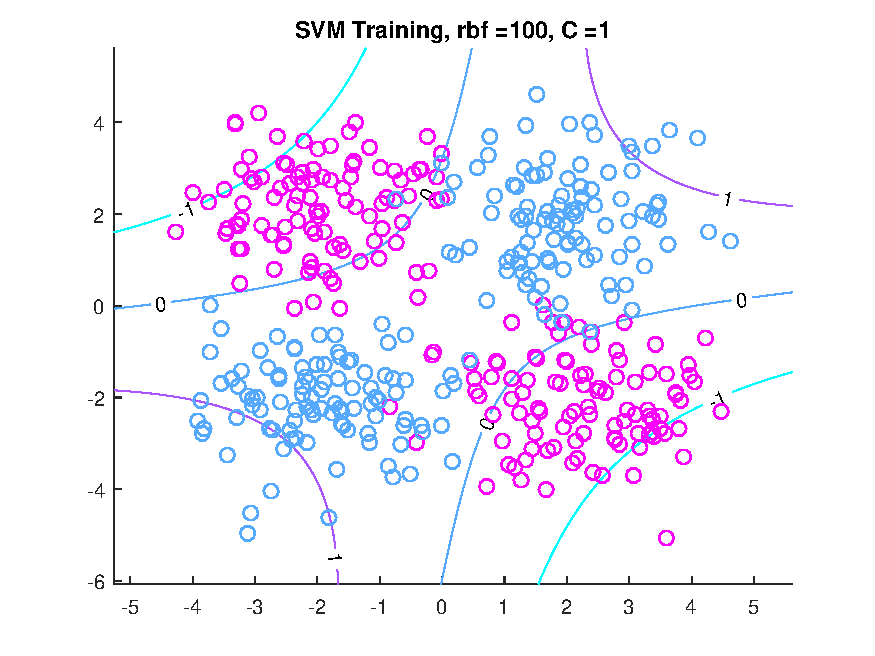
\includegraphics[scale=0.4]{figures/hw2_2_nonsep_rbf_100_a_1.pdf}
	\caption{$\sigma^2$ = 100}\label{fig:svm_data_nonsep_a}
    \end{subfigure}  
    \caption{Plots of decision boundaries from SVM with gaussian kernel, $C=1$ on ``nonsep'' dataset, varying values of the bandwidth parameter.}  \label{fig:SVM_kernel_plots}  
\end{figure}

{\bf Questions:}
\begin{enumerate}[label=(\alph*)]
	\item As $C$ increases, the geometric margin $1/\|\V{w}\|$ decreases.  If the data is not linearly separable, then
	the geometric margin $1/\|\V{w}\|$ decreases strictly monotonically as $C$ increases.  However, if the data is linearly
	separable, then this does not always happen as we increase $C$.  In this case, once the margin is sufficiently small
	such that all points are correctly classified, then it will not decrease further even as $C$ approaches infinity.  
	
	\item As $C$ increases, the number of support vectors generally decreases.  This is because the larger penalty on misclassified
	points leads to a decision boundary with fewer misclassifications on the training data.  The number of the
	support vectors is bounded below by two as $C$ approaches infinity, because there will always be at least one support vector
	on each side of the decision boundary.  However, there are pathological examples where the number of support vectors increases as $C$ increases for some values, which we observe for the nonseparable dataset.  
	
	\item Maximizing the geometric margin $1/\|\V{w}\|$ on the training data is not an appropriate criterion for selecting
	$C$ because this leads to a classifier which is overfit to the training set.  To obtain a classifier which generalizes well
	on test data, we should use out-of-sample data to select an appropriate value for $C$.  To do this, we can train the SVM model
	with $C = \{0.01,0.1,1,10,100\}$, and then select the value for $C$ which yields the classifier with the highest
	accuracy on the validation set.  

\end{enumerate}

%TODO: continue